\begin{frame}
\frametitle{Il codice}
\begin{block}{Primi passi verso l'implementazione}
Abbiamo avuto modo di analizzare un prototipo scritto in \textsc{Matlab}
\end{block}

\begin{block}{}
\begin{itemize}
\item Analisi del codice
\item Creazione \emph{workflow}
\item Associazione tra \emph{workflow} del codice modello teorico
\item \textit{Debugging} e \textit{refactoring} del codice
\end{itemize}
\end{block}

\begin{block}{}
Parallelamente \`e stata portata avanti una ristesura del codice, in \emph{Python}
e \emph{OpenCV}, da usare come base per sviluppi futuri
\end{block}
\end{frame}

\begin{frame}
\frametitle{Workflow}
\begin{figure}
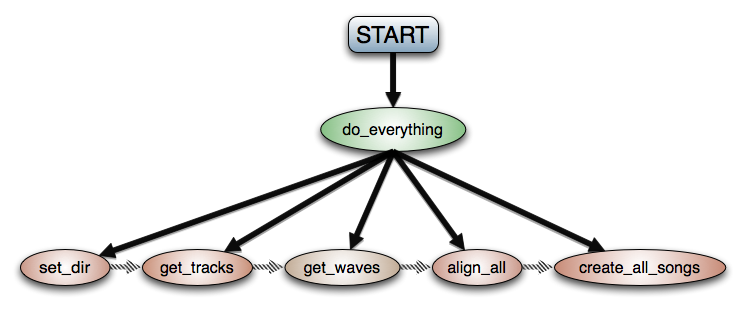
\includegraphics[width=\textwidth]{immagini/workflow.png}
\end{figure}
\end{frame}

